\textbf{
    Construya el árbol de Huffman para codificar el siguiente texto:
    \begin{center}
        "El azote, hijo mío, se inventó para castigar afrontando al racional y para avivar la pereza del bruto que carece de razón; pero no para el niño decente y de vergüenza que sabe lo que le importa hacer y lo que nunca debe ejecutar, no amedrentado por el rigor del castigo, sino obligado por la persuasión de la doctrina y el convencimiento de su propio interés."
    \end{center}
}\vspace{.2cm}

No voy a explicar el algoritmo de Huffman, pues se vio en clase pero voy a hacer el procedimiento y luego mostrar con un árbol de Huffman online que esta bien hecho. \vspace{.2cm}

\textcolor{bibi}{Creamos el arbol de Huffman}
\begin{quote}
    \begin{itemize}
        \item \textbf{Paso 1:} Contamos la frecuencia de cada letra en el texto. (puede cambiar un poquito si consideras tabuladores o si yo conte mal xd)

        \begin{align*}
            \char`_ &: 65 \\
            e &: 39 \\
            a &: 34 \\
            o &: 27 \\
            r &: 25 \\
            n &: 21 \\
            i &: 17 \\
            l &: 15 \\
            t &: 13 \\
            d &: 13 \\
            c &: 12 \\
            p &: 11 \\
            s &: 9 \\
            u &: 9 \\
            v &: 5 \\
            g &: 5 \\
            z &: 4 \\
            , &: 4 \\
            m &: 4 \\
            y &: 4 \\
            b &: 4 \\
            q &: 4 \\
            \text{ó} &: 3 \\
            h &: 2 \\
            j &: 2 \\
            E &: 1 \\
            \text{í} &: 1 \\
            f &: 1 \\
            ; &: 1 \\
            \text{ñ} &: 1 \\
            \text{ü} &: 1 \\
            \text{é} &: 1 \\
            . &: 1 \\
        \end{align*}
        \item \textbf{Paso 2:} Creamos una lista con los nodos de cada letra y su frecuencia. (este paso literalmente solo es hacer eso entonces no muestro nada)
        \item \textbf{Paso 3:} Tomamos 2 arboles con las frecuencias mas bajas y los unimos en un nuevo arbol con la suma de las frecuencias, la raiz de este nuevo arbol es la suma de las frecuencias y los hijos son los arboles que unimos. Ademas, se etiqueta cada rama con un 0 si esta a la izquierda o un 1 si esta a la derecha, (este paso es el mas largo y tedioso, asi que solo muestro el resultado final)
        \item \textbf{Paso 4:} Repetimos el paso 3 hasta que solo quede un arbol. \vspace{.2cm}
    \end{itemize}

    No se si no se podia pero yo utilice un graficador en linea, igualmente el link del graficador es \href{https://www.csfieldguide.org.nz/en/interactives/huffman-tree/}{\underline{este}} y el resultado es este: \vspace{.2cm}

    \textbf{NOTA:} El graficador no le importa tanto si es izquierda o derecha al a hora de mostrar el resultado grafico (por eso aveces pone 0 a la derecha) pero internamente si lo esta haciendo solo lo dibuja al reves. \vspace{.2cm}
    \begin{center}
        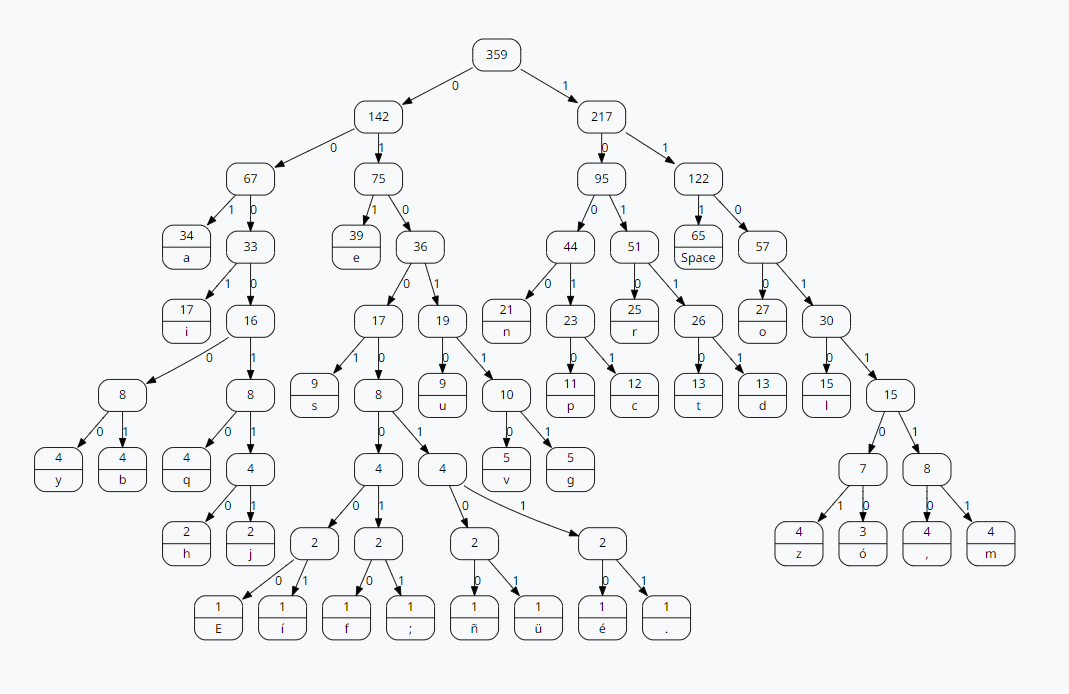
\includegraphics[width=14.9cm]{src/Img/ArbolHuffman.png}
    \end{center}

    Pero bueno por si acaso lo explico un poquito, hasta abajo vemos que los de frecuencia 1 se empezaron uniendo entre si generando arboles con raiz 2, a su vez se unieron entre si para generar arboles con raiz 4, aveces, cuando no hay arboles con la misma raiz, se toman los 2 de menor raiz digamos 8 y 9 se juntan para una raiz 17, y asi sucesivamente hasta que solo queda un arbol de raiz 359. \vspace{.2cm}

    Ahora, como mencionamos ir a la izquierda desde la raiz agrega un 0 a la codificacion del caracter y a la derecha un 1, entonces, si queremos saber la codificacion de una letra, simplemente seguimos el camino desde la raiz hasta la letra y anotamos los 0s y 1s que tomamos, este camino es unico aunque la codificacion no lo sea  (existen varias codificaciones de Huffman para este texto). Entonces por ejemplo el espacio tiene 111 como codificacion mientras que el . tiene una codificacion de 01000111 \vspace{.2cm} 
\end{quote}